%\rowcolors{0}{}{}
%\begin{figure}[!htb]
\centering
\def\firstcircle{(-3, 1.5) circle (3.5)} % Lógico
\def\secondcircle{(-0.5, 1.5) circle (3)} % Físico
\def\thirdcircle{(-2.3, -1.5) circle (2.5)} % Conceitual
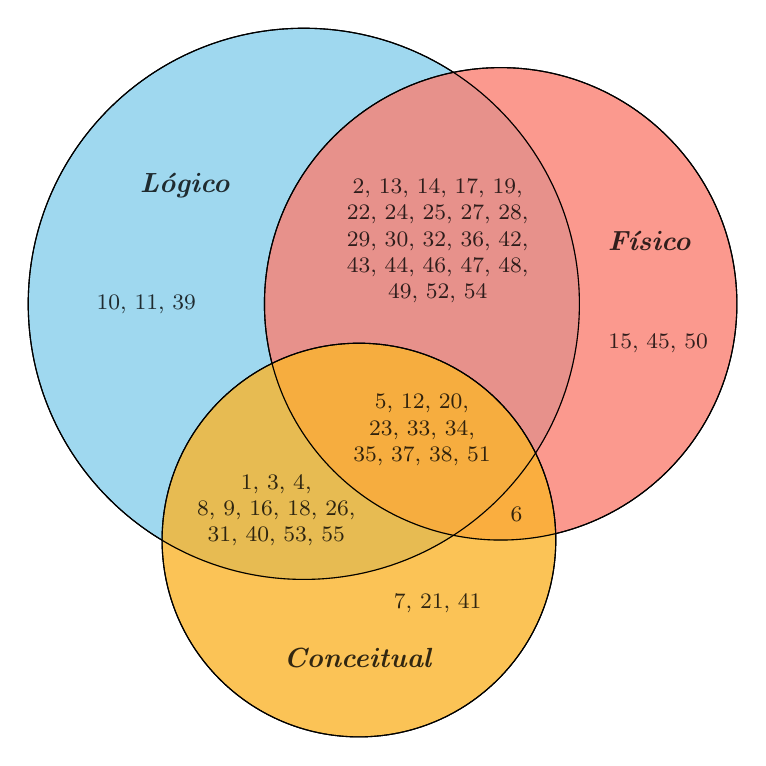
\begin{tikzpicture}
\centering
\begin{scope}[shift={(4cm,-15cm)}, fill opacity=.8]
        \fill[SkyBlue, draw = black] \firstcircle;
        \fill[Salmon, draw = black] \secondcircle;
        \fill[Dandelion, draw = black] \thirdcircle;
        \draw \firstcircle node at(-1.3, -2.3) {
        \footnotesize
        \begin{tabular}{c}
        %\textbf{CONCEITUAL} \\ %Conceitual
         7, 21, 41
        \end{tabular}
        };
        \draw \secondcircle  node at(-5, 1.5) %[text width=5cm,align=center] 
        {
        \footnotesize
        \begin{tabular}{c}
        %\textbf{LÓGICO} \\ %Lógico
        10, 11, 39
        \end{tabular}
        };
        \draw \thirdcircle node at(1.5, 1) %[text width=2.7cm,align=center] 
        {
        \footnotesize
        \begin{tabular}{c}
        %\textbf{FÍSICO}\\ %Físico
        15, 45, 50
        \end{tabular}
        };
        \draw node at(-3.35 ,-1.12) { 
        \footnotesize
        \begin{tabular}{c} 
        %Conceitual + Lógico
        1, 3, 4,\\
        8, 9, 16, 18, 26,\\
        31, 40, 53, 55
        \end{tabular}
        };
        \draw node at(-1.5, -0.1) { 
        \footnotesize
        \begin{tabular}{c} 
        %Conceitual + Lógico + Físico
        5, 12, 20,\\
        23, 33, 34,\\
        35, 37, 38, 51
        \end{tabular}
        };
        \draw node at(-1.3, 2.3) { 
        \footnotesize
        \begin{tabular}{c} 
        %Lógico + Físico
        2, 13, 14, 17, 19,\\
        22, 24, 25, 27, 28,\\
        29, 30, 32, 36, 42,\\
        43, 44, 46, 47, 48,\\
        49, 52, 54
        \end{tabular}
        };
        \draw node at(-0.3, -1.2) { 
        \footnotesize
        \begin{tabular}{c} 
        %Conceitual + Físico
        6
        \end{tabular}
        };
        
    \node at (-4.5,3) {\textit{\textbf{Lógico}}};
    \node at (1.4,2.3) {\textit{\textbf{Físico}}};
    \node at (-2.3,-3) {\textit{\textbf{Conceitual}}};
    
    %\begin{scope} %Código para as interseções
    %    \clip \firstcircle;
    %    \fill[lightgray] \secondcircle;
    %\end{scope}
    
    \end{scope}
\end{tikzpicture}
%\caption{Diagrama de Venn dos modelos suportados nas ferramentas.}
%\label{fig:VennDiagram}
%\end{figure}